% Apostel, Bogdanski, Ritter
%
% Wahlpflichtfach Künstliche Intelligenz:
% Projekt - Schiffe Versenken
%
% Hochschule Bremen - University of applied siences
% ============================================================================
%
% report.tex
%
% das Wurzel-Dokument, fügt alle einzelteile zusammen

%!TEX root = /Users/stefanbogdanski/Dropbox/BÄTTLESHÖP/Dokumentation/dokumentation.text
% 
% Apostel, Bogdanski, Ritter
%
% Wahlpflichtfach Künstliche Intelligenz:
% Projekt - Schiffe Versenken
%
% Hochschule Bremen - University of applied siences
% ============================================================================
%
% header.tex
%
% Präambel und LaTeX Einstellungen

\documentclass[
    pdflatex,           % Use PDFTex
    a4paper,            % A4 paper
    oneside,            % oneside print
    12pt,               % Font size 12pt
    captions=tableheading,  % korrekte Abstaende bei TabellenUEBERschriften
    chapterprefix,      % Chapter write to as chapter
    headsepline,        % Line after header
    footsepline,        % Line before footer
    headinclude,        % Kopfzeile wird Seiten-Layouts mit beruecksichtigt
    footinclude=false,  % Fu{\ss}zeile wird Seiten-Layouts mit 
    plainheadsepline,   % horizontale Linie auch beim plain-Style
    fleqn,              % Write the formula left-aligned
    appendixprefix,
	bibtotocnumbered,	%referencen mit nummerieren und ins inhalts VZ 
]{scrartcl}
\usepackage{graphicx}
\usepackage{graphics}
\usepackage{epsf}
\usepackage{epsfig}
\usepackage{amsmath}
%
% package for the appendix.
%
\usepackage{appendix}

% mehrzeilige Captions ausrichten
\usepackage[font=footnotesize]{caption}
%
% package to create subfigure, subtables
%
\usepackage{subfigure} 

%
%package to include pdf-files to Latex Document
%
\usepackage{pdfpages}

%
% package for the index.
%
\usepackage{makeidx} 

\usepackage{rotfloat}



%
% using babel
%
\usepackage[ngerman]{babel}

%
% package to use the UTF8 character and their writings
%
\usepackage[utf8]{inputenc}
%\usepackage[T1]{fontenc}
\usepackage{textcomp}

%
% Flie{\ss}umgebung: Erm\"{o}glicht Platzierung [H] f\"{u}r Grafiken und Tabellen
%
\usepackage{float}
\restylefloat{figure}
\restylefloat{table}

%
% package for more table settings
%
\usepackage{array}%,tabularx}
%\usepackage[table,svgnames]{xcolor}
\usepackage{ragged2e}

\usepackage{setspace}            % Zeilenabstand einstellbar
\onehalfspacing                  % eineinhalbzeilig einstellen

\typearea[current]{current}        % Neuberechnung des Satzspiegels mit alten Werten nach \"{A}nderung von Zeilenabstand,etc


%
% header und footer
%
%\pagestyle{headings}
%\usepackage{scrpage2}            % Kopf und Fusszeilen-Layout
\renewcommand{\headfont}{\normalfont\sffamily}    % Kolumnentitel serifenlos
\renewcommand{\pnumfont}{\normalfont\sffamily}    % Seitennummern serifenlos
%\pagestyle{headings}
%\ihead[]{\headmark}              % Kolumnentitel immer oben innen
%\ohead[\pagemark]{\pagemark}     % Seitennummern immer oben aussen
%\ofoot{\pagemark}                       % Seitennummern in der Fusszeile loeschen

\usepackage[automark]{scrpage2}
\ihead{}
\ohead{\headmark}
\chead{}
\cfoot{}
\ofoot{\pagemark}

\pagestyle{scrheadings}

% 
\usepackage{blindtext}
% define the color "LinkColor"
%
\definecolor{LinkColor}{rgb}{1,0,0}
\definecolor{CiteColor}{rgb}{0,1,0}
\definecolor{URLColor}{rgb}{0,0,1}

%
% package for using Hyperlinks in PDF files
%
 \usepackage[
	pdftitle={Projekt - Schiffe Versenken},
	pdfauthor={Apostel, Bogdanski, Ritter},
	pdfsubject={Wahlpflichtfach KI},
	plainpages=true
    ]{hyperref}
\hypersetup{colorlinks=false,
	linkcolor=LinkColor,
	citecolor=CiteColor,
	filecolor=LinkColor,
	menucolor=LinkColor,
%	pagecolor=LinkColor,
	urlcolor=URLColor}

%
% package to represent listings in their formats
%

\usepackage[colorinlistoftodos]{todonotes}
\newcommand{\todoin}[1]{\todo[inline]{#1}}

%
% package to use the abstract environment
%
\usepackage{abstract}

%
% package to use URLs
%
\usepackage{url}
\usepackage{listings} 
\usepackage{color}   

%
% build index
%
\makeindex

%
% build glossary
%
\makeglossary

%\usepackage[savemem]{listings}

\begin{document}
	\listoftodos
	\pagenumbering{Alph}
		%!TEX root = /Users/stefanbogdanski/Dropbox/BÄTTLESHÖP/Dokumentation/dokumentation.tex
%
% Apostel, Bogdanski, Ritter
%
% Wahlpflichtfach Künstliche Intelligenz:
% Projekt - Schiffe Versenken
%
% Hochschule Bremen - University of applied siences
% ============================================================================
%
% 0_deckblatt.tex
%
% Beschreibung des Dateiinhalts
\begin{titlepage}
	\begin{figure}[lt] % (fold)
		
\includegraphics[scale=0.5]{images/logo_a4.pdf}
	\end{figure}
	% figure figure label (end)
	\begin{Center}
		\Huge
		Wahlpflichtfach KI\newline
		\vspace*{1cm}
		\Large
		Projektdokumentation: Schiffe Versenken
	\end{Center}	
	\vfill
	\begin{table}[H] % (fold)
		\centering
		\begin{tabular}{ll}
			Autoren: & Victor Apostel, Stefan Bogdanski, Sibille Ritter \\
			Studiengang: & (Internationaler) Studiengang Technische Informatik B.Sc. \\
		\end{tabular}
		\label{label}
	\end{table}
	\todoin {Liebe Gruppenmitglieder, \newline so langsam müssen wir auch bedenken, dass dieses Dokument nicht den Rahmen sprengen darf. m.E. ist es bereits viel zu lang! Der Inhalt ist - wie zu erwarten - auf einem sehr schönen qualitativen Niveau. Aber man darf es hier nicht aus den Fugen laufen lassen. Denkt daran, dass der 'arme' Prof. Breymann das auch alles lesen muss. Wir haben inzwischen ein fast 40(!!!) seitiges Pamphlet zu einer Implementierung von Schiffe versenken verfasst.\newline Ich bin mir bewusst, dass mein Anteil an diesem Dokument der geringste ist, und ich will mich bei Leibe nicht darüber beschweren, dass soviel von euch geschrieben wurde! Aber trotzdem möchte ich apellieren, dass der Rahmen m.E. bereits überschritten ist und nun die Zeit gekommen ist auf die bremse zu treten. Dies ist keine Bachelor-Thesis, dies ist ein WPM. LG, HEGDL und alles! - SB}
\end{titlepage}
	\pagenumbering{roman}
		%\include{chapters/02_abstract}
	\pagenumbering{arabic}
		\include{toc}
		\listoffigures 
		\listoftables
		\clearpage 
		%\input{chapters/1_chapter}
		\section{Einleitung}
\label{sec:Einleitung}
	\todo{detaillierte Aufgabenbeschreibung}
		\section{Spielregeln}
\label{sec:Spielregeln}

Da die allgemeinen Regeln des Spiels \textit{Schiffe versenken} bekannt sein sollten, werden an dieser Stelle nur die relevanten Eckdaten aufgeführt:

\todo{Vervollständigen}

\begin{itemize}
	\item Spielfelder
		\begin{itemize}
			\item 10 x 10 Felder gross
			\item Eigenes Feld entweder: Wasser, Schiff, Getroffen
			\item Gegnerisches Feld entweder: Unbekannt, Treffer, Versenkt
		\end{itemize}
	\item Schiffe
		\begin{itemize}
			\item 1 x 5er, 1 x 4er, 2 x 3er, 1 x 2 er
			\item Schiffe dürfen sich nicht berühren
		\end{itemize}
	\item Spielablauf
		\begin{itemize}
			\item Die beiden Spieler schießen abwechselnd bis sämtliche Schiffe eines Spielers versenkt sind.
		\end{itemize}
	
\end{itemize}
		\section{Kommunikationsmodell}
\label{sec:Kommunikationsmodell}

		\section{Softwarearchitektur}
\label{sec:Softwarearchitektur}

Die Software des Spiels "'Schiffe versenken"' wurde als Client-Server Anwendung gemäß Abbildung \ref{fig:Kommunikationsteilnehmer} entworfen.
Die zentrale Kommunikationsschnittstelle stellt der Kommunikationsserver dar, der auf dem Port $54321$ eingehende Verbindungen annimmt.
Verbindungen können sowohl mittels eines Java-Clients hergestellt werden, die von einem Menschen bedient werden, als auch von Prolog-Clients, die vollständig autonom agieren.
Es liegen hinsichtlich der Clientkombinationen keine Beschränkungen vor, sodass auch z.B. ein Prologclient gegen einen anderen Prologclient antreten kann.

\begin{figure}[H]
  \centering
  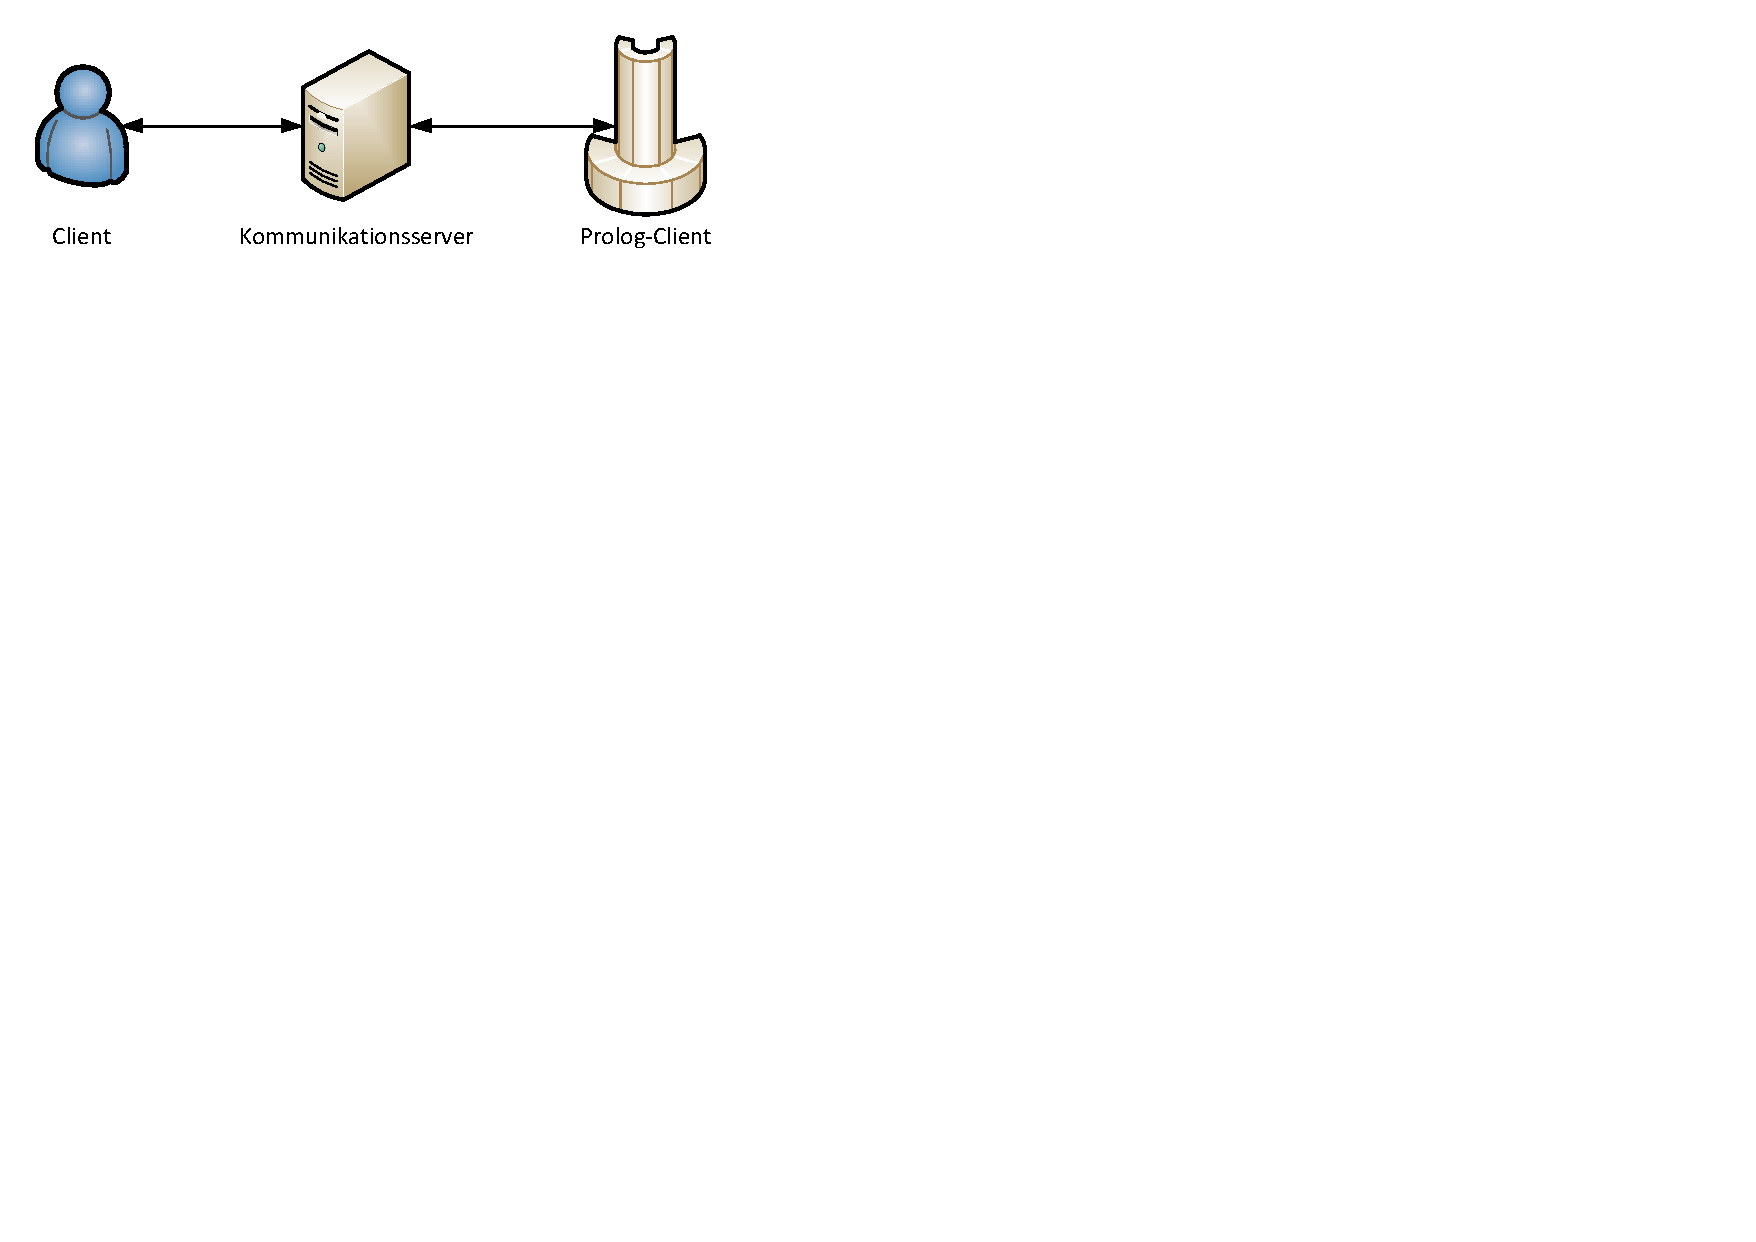
\includegraphics[trim=0mm 165mm 175mm 0mm,clip,width=0.5\textwidth]{images/Kommunikationsmodell.pdf}
  \caption{Darstellung der möglichen Kommunikationsteilnehmer}
  \label{fig:Kommunikationsteilnehmer}
\end{figure}

Der gesamte Spielverlauf lässt sich anhand der Statusdiagramme in den Abbildungen \ref{fig:Clientstates} und \ref{fig:SubClientstates} beschreiben.
Diese sind sowohl für den Javaclient, als auch für das Prologprogramm gültig.

Unmittelbar nach Start des Clients befindet sich dieser im Initialisierungszustand \emph{INITIALIZATION}.
Während dieser Phase obliegt es dem Client seine Schiffe gemäß den Regeln zu platzieren.
Des Weiteren hat er eine Nachricht des Servers zu empfangen, die angibt, ob sein initialer Zustand \emph{DEFENCE} oder \emph{ATTACK} sein soll, wenn er in die \emph{RUNNING}-Phase übergeht.
Dieser Übergang erfolgt durch den Empfang des Startkommandos, mit dem Opcode = 5.

\begin{figure}[H]
  \centering
  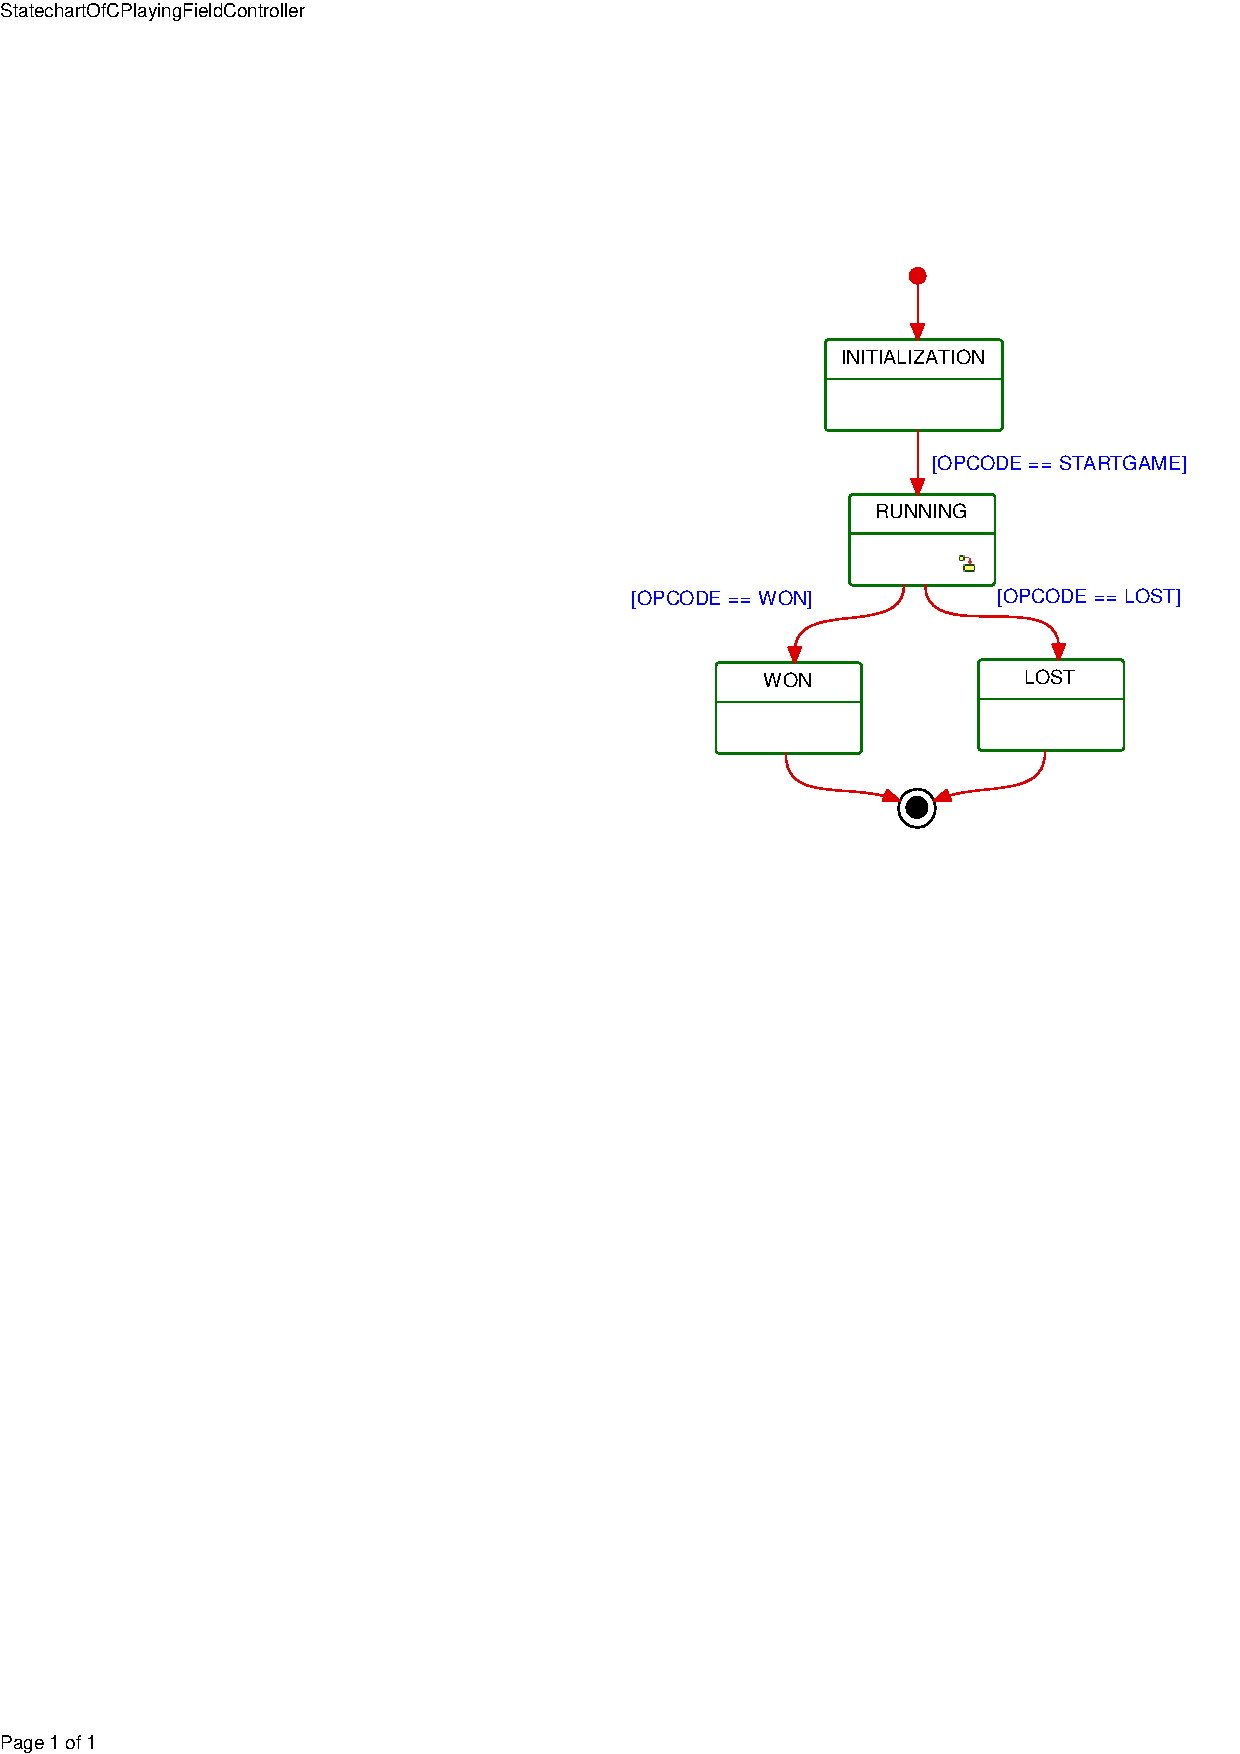
\includegraphics[trim=105mm 155mm 5mm 42mm,clip,width=0.5\textwidth]{images/SMController.pdf}
  \caption{Zustandsübergänge des Clients}
  \label{fig:Clientstates}
\end{figure}

Befindet sich der Client im \emph{RUNNING}-Status, so wechselt er zwischen seinen internen Zuständen \emph{ATTACK} und \emph{DEFENCE} hin und her.
Dieser Wechsel erfolgt immer dann, wenn eine \emph{ATTACKRESPONSE} Nachricht mit dem Opcode = 2 übertragen wurde.
Der primäre Unterschied zwischen beiden Zuständen ist die Reihenfolge der erwarteten Nachrichten.
Befindet sich der Client im Subzustand \emph{DEFENCE}, so erwartet er von seinem Kontrahenten eine Nachricht mit dem Opcode = 1 und beantwortet diese seinerseits mit dem Opcode = 2.
Sollte sich der Client im Subzustand \emph{ATTACK} befinden, so sendet er zuerst die Nachricht mit dem Opcode = 1 und erwartet im Anschluss eine Nachricht seines Gegners.

Das Alternieren der Zustände erfolgt solange, wie in der Antwortnachricht mit dem Opcode = 2 keine Meldung über den Verlust aller Schiffe transferiert wird.
Dieses Ereignis wird gemäß Tabelle \ref{tbl:Ergebniskodierung} auf Seite \pageref{tbl:Ergebniskodierung} mit dem Ergebniscode = 4 beschrieben.
Empfängt der Client die Nachricht, so gilt das Spiel als gewonnen.
Umgekehrt verliert der Client das Spiel, wenn er diese Nachricht verschickt.

Im Rahmen dieses Kontexts wechselt der Spielzustand in \emph{WON} bzw. \emph{LOST} und das Programm kann beendet werden.

\begin{figure}[H]
  \centering
  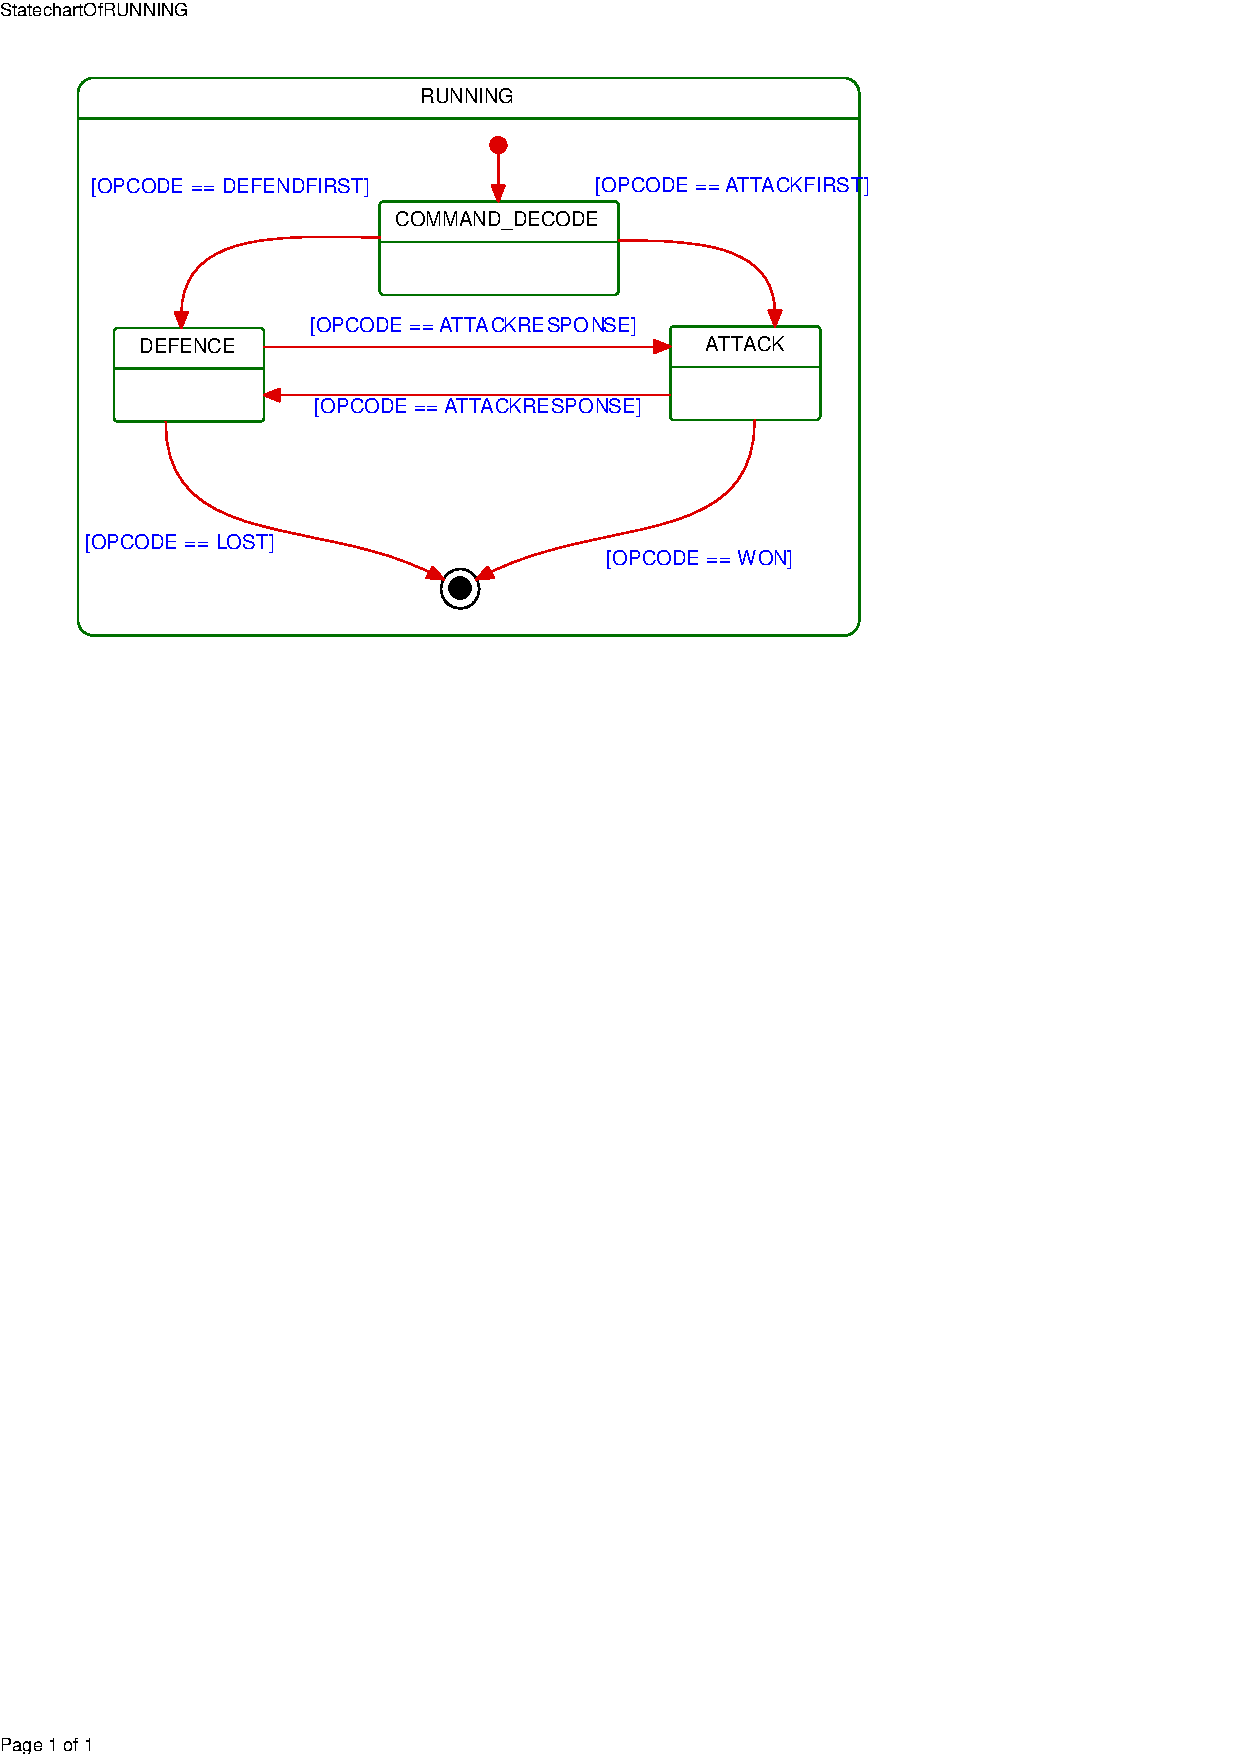
\includegraphics[trim=10mm 185mm 60mm 10mm,clip,width=0.5\textwidth]{images/SubSMRUNNING.pdf}
  \caption{Interne Zustandsübergänge während des laufenden Spiels}
  \label{fig:SubClientstates}
\end{figure}

Die vorgesehene Kommunikationsabfolge wird ebenfalls in Abbildung \ref{fig:Kommunikationssequenz} in Form eines Sequenzdiagramms dargestellt.
Der Client, der sich zuerst mit dem Server verbindet, beginnt per Konvention im Verteidungsmodus und der zweite verbundene Client startet im Angriffsmodus.
Erst wenn sich zwei Teilnehmer am Server verbunden haben, sendet dieser das Startsignal an alle Clients.

Die Spielphase wird durch eine Schleife bestimmt, in der die Teilnehmer von den Angriffs- in den Verteidigungszustand wechseln und umgekehrt.
Die dabei übertragenen Nachrichten werden stets an den Server übertragen, der diese an den zweiten Client weiterleitet.
Dadurch kommt keine direkte Verbindung beider Spieler zustande.

Das Programmende aus Sicht der Kommunikation wird erreicht, wenn ein Spieler die Nachricht überträgt, dass er über keine Schiffe mehr verfügt.
In diesem Fall werden die Verbindungen getrennt und der Server kann neue Verbindungen von Spielern zum Ausrichten eines neuen Spiels annehmen.

\begin{figure}[H]
  \centering
  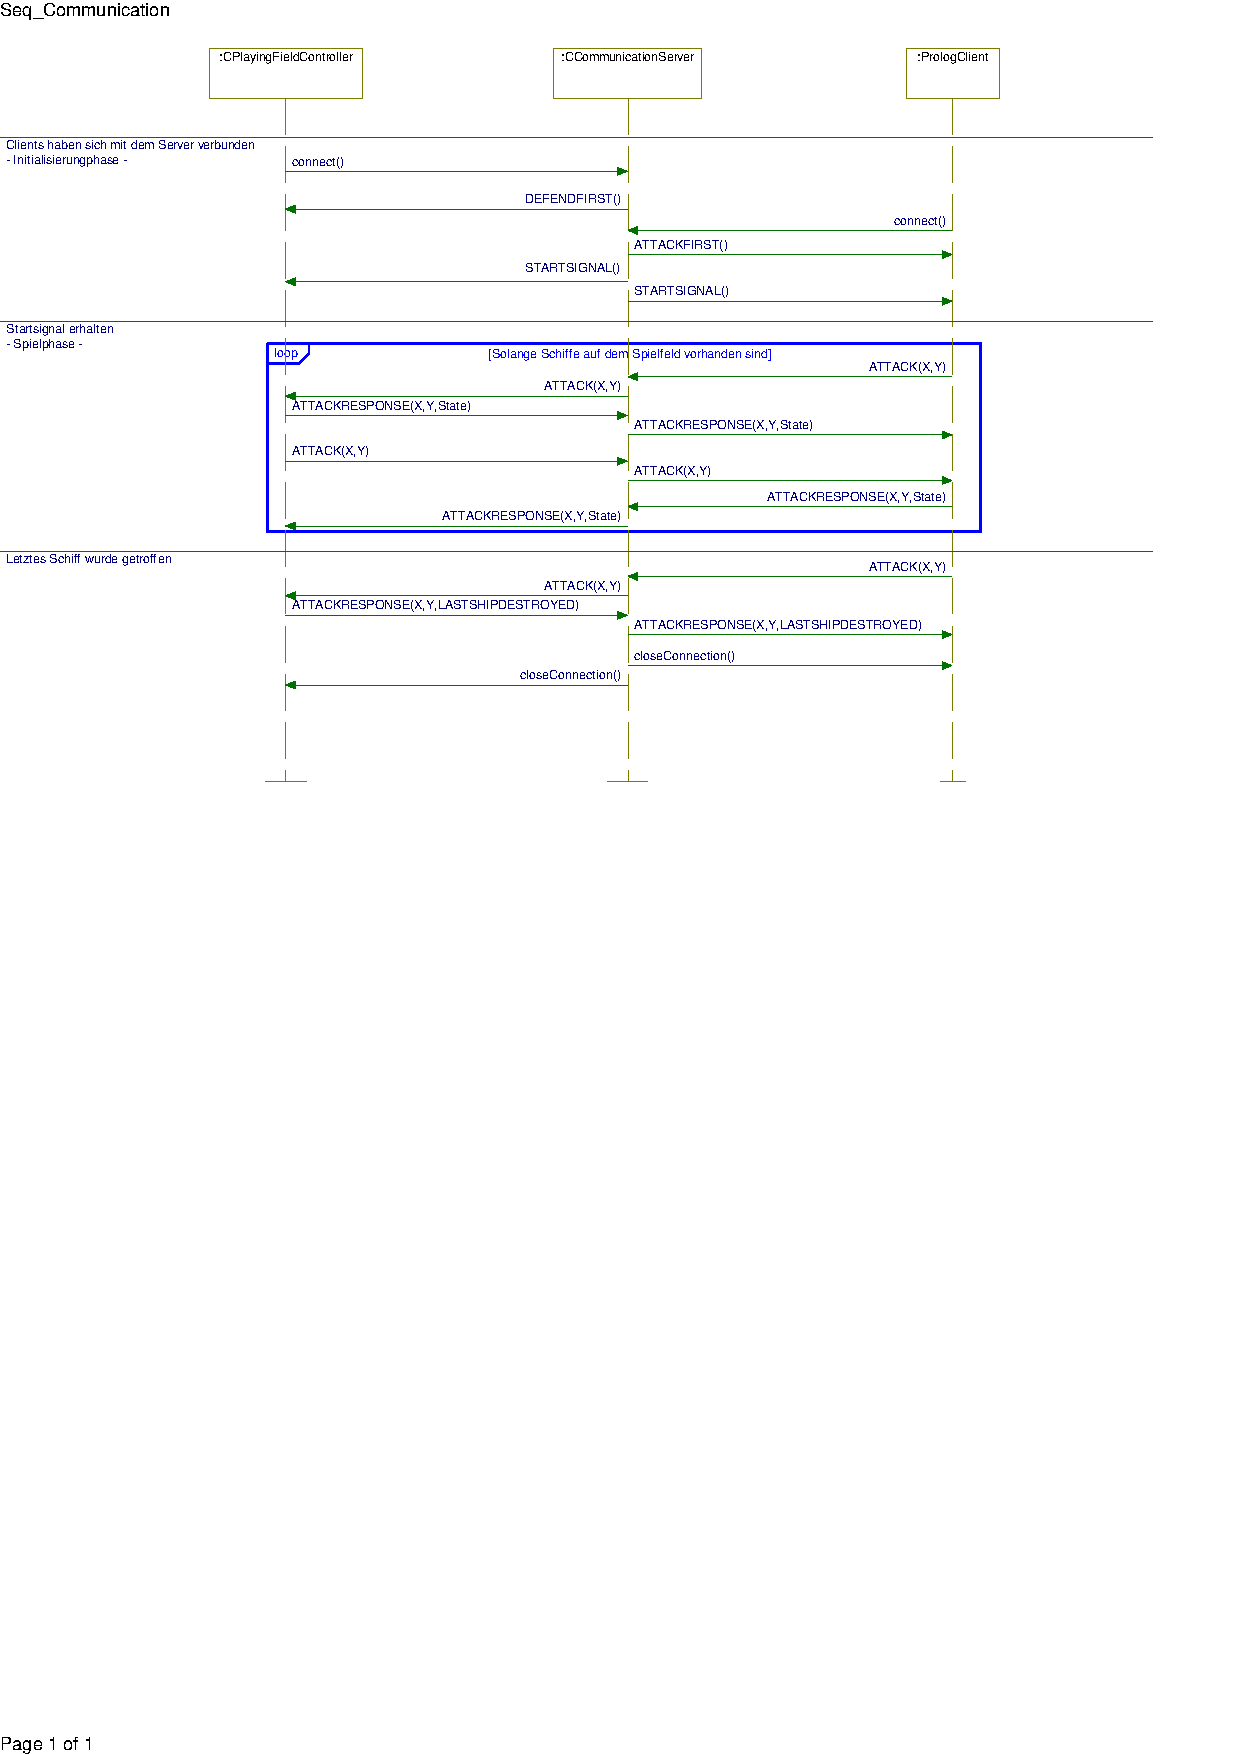
\includegraphics[trim=0mm 160mm 25mm 5mm,clip,width=0.9\textwidth]{images/SeqCommunication.pdf}
  \caption{Sequenzdiagramm der Kommunikation}
  \label{fig:Kommunikationssequenz}
\end{figure}


		\subsection{Spielserver}
\label{sec:Spielserver}

Der Server bildet die Schnittstelle zwischen den beiden Kommunikationspartnern, indem er eingehende Nachrichten eines Clients an jeden anderen verbundenen Teilnehmer weiterleitet.
Des Weiteren limitiert er die maximale Spielerzahl und generiert das Startsignal, sobald sich zwei Teilnehmer mit ihm verbunden haben.
Außerdem legt das Programm fest, welcher der Spieler im Verteidigungs- bzw. Angriffsmodus startet.

Die Serverlogik wird maßgeblich durch die beiden Klassen \texttt{CCommunicationServer} und \texttt{CClientHandler} gesteuert (vgl. Abbildung \ref{fig:Serverklassendiagramm}).
Die Aufgabe der Klasse \texttt{CCommunicationServer} ist die Annahme eingehener Verbindungen.
Für jeden verbundenen Client wird ein separater Thread vom Typ \texttt{CClientHandler} erzeugt und gestartet.

Diese Threadobjekte führen die eigentliche Serverlogik aus.
Sie überwachen den eingehenden Datenstrom und sobald eine Nachricht eingegangen ist, wird diese kopiert und an jeden anderen Client weitergeleitet.
Für die Überwachung des Eingangsstromes ist die Methode \texttt{run()} verantwortlich und das Duplizieren der Nachricht wird in \texttt{notifyAllOtherClients(String line)} gehandhabt.
Der eigentliche Sendevorgang wird durch den Aufruf der Methode \texttt{send(String msg)} ausgeführt.

\begin{figure}[H]
  \centering
  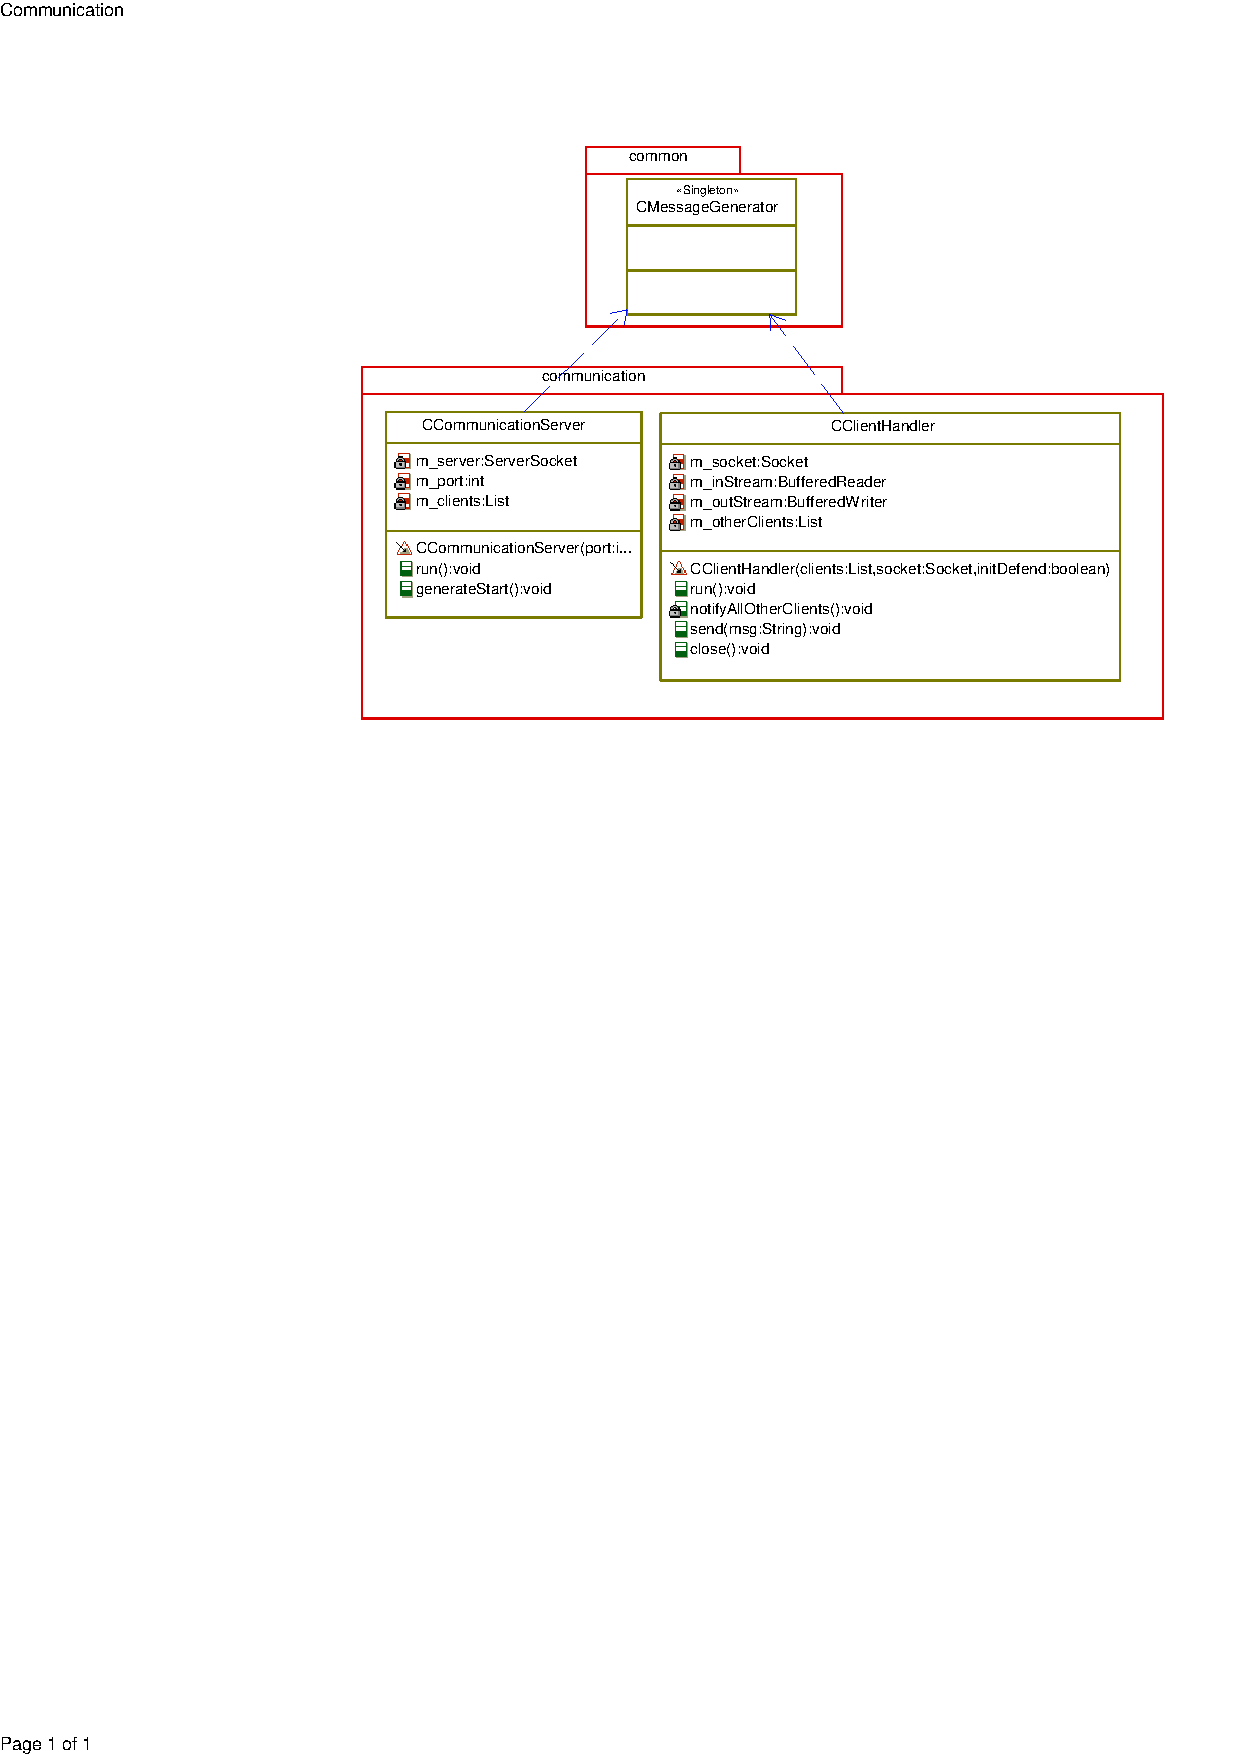
\includegraphics[trim=60mm 165mm 10mm 20mm,clip,width=0.8\textwidth]{images/Server.pdf}
  \caption{Klassendiagramm des Servers}
  \label{fig:Serverklassendiagramm}
\end{figure}

		\subsection{Client - Java}
\label{sec:Javaclient}

Der hier beschriebene Javaclient ist ein möglicher Teilnehmer, der sich mit den Kommunikationsserver verbinden und ein Spiel austragen kann.
Sein Design orientiert sich am Model-View-Controller Prinzip, wobei das Spielbrettmodell auf Grund seines geringen Umfangs im Controller eingebettet wurde.

Eine Übersicht des Entwurfs wird in Abbildung \ref{fig:Javaclientklassendiagramm} dargestellt.


\begin{figure}[H]
  \centering
  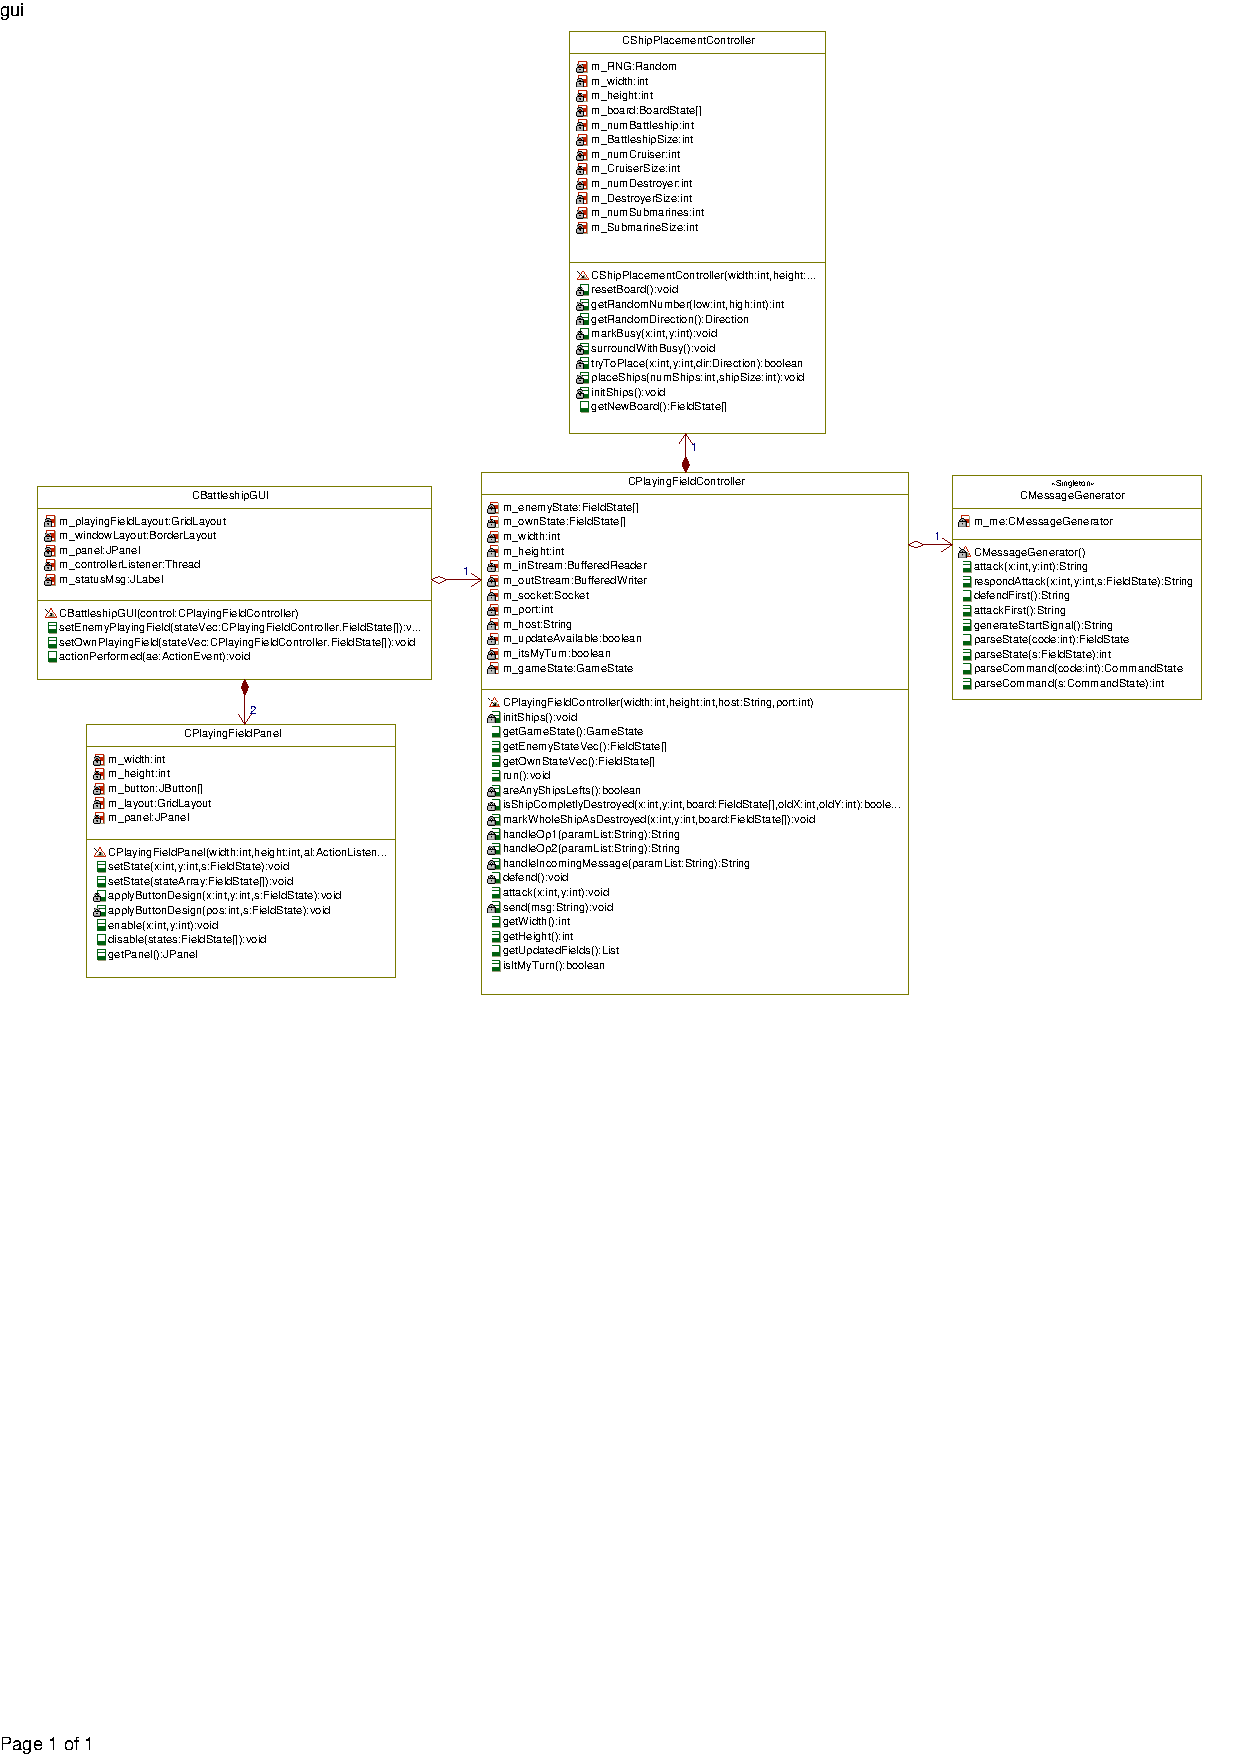
\includegraphics[trim=5mm 125mm 5mm 4mm,clip,width=0.9\textwidth]{images/CJavaClient.pdf}
  \caption{Klassendiagramm des Java Clients}
  \label{fig:Javaclientklassendiagramm}
\end{figure}

		\subsection{Client - Prolog} \label{sec:Prologclient}
	Die Aufgaben des Prolog-Clients sind in verschiedene Module unterteilt, um die verschiedenen Teile austauschbar zu halten. 
	Im Folgenden werden die Aufgaben und die Funktionsweise dieser Module erläutert.
	
	\todo{Gesamtübersicht - Bild - Modulzusammenspiel?}



\subsubsection{Hauptmodul}
	Das Hauptmodul \texttt{main.pl} wird beim starten des Clients aufgerufen. Das Modul initialisiert zunächst die Verbindung zum
	Spielserver. Anschließend werden Spielvorbereitungen über das Prädikat \texttt{initPrologClient/0} aus dem 
	Initialisierungsmodul getroffen (siehe Abschnitt \ref{sec:initModule}).
	
	Je nachdem ob der Client im Angriffs- oder Verteidigungsmodus startet, werden die Prädikate \texttt{attackFirst/0} oder
	\texttt{defendFirst/0} aufgerufen. Nach Empfang des Startsignals beginnt der Client dann mit einem Angriff oder Verteidigung.
	
	Ein Angriff verwendet die Prädikate \texttt{doAttack/2} und \texttt{attackResponse/3} des Angriffsmoduls (siehe Abschnitt
	\ref{sec:attackModule}).
	Das Prädikat \texttt{doAttack/2} liefert den Punkt auf dem gegnerischen Spielfeld der angegriffen werden soll.
	Die so erhaltenen X-Y-Koordinaten gibt das Hauptmodul an den Server weiter und wartet anschließend auf eine Antwort des 
	Gegners (über den Server). 
	Nach Erhalt dieser Antwort verwendet das Hauptmodul das Prädikat \texttt{attackResponse/3}, um die Antwort zu verarbeiten.
	Mit Abschluss der Verarbeitung ist der Angriff beendet.
	
	Die Verteidigung verwendet das Prädikat \texttt{doDefend/3} des Verteidigungsmoduls (siehe Abschnitt \ref{sec:defendModule}).
	Zu Beginn der Verteidigung wartet das Hauptmodul zunächst auf den Angriff des Gegners. Die so erhaltenen Koordinaten
	werden an das Prädikat \texttt{doDefend/3} übergeben. Als Resultat liefert dieses Prädikat die entsprechende Antwort für den
	Gegner. Das Hauptmodul sendet die Antwort gemäß dem Kommunikationsprotokoll an den Server. Damit ist die Verteidigung 
	beendet.
	
	Nach jedem Angriff überprüft der Client, ob er das Spiel gewonnen hat. Gleichermaßen überprüft er nach jeder Verteidigung, 
	ob er das Spiel verloren hat. Tritt einer der beiden Fälle in Kraft, so beendet sich der Client mit einer der beiden Ausgaben
	\textit{KI wins. End of game.} oder \textit{KI looses. End of game.}.
	

\subsubsection{Initialisierungsmodul} \label{sec:initModule}
	Die Aufgaben des Initialisierungsmoduls \texttt{initModule.pl} sind das initialisieren der Spielfelder, darunter auch
	das Platzieren der eigenen Schiffe. Hierzu werden die Prädikate \texttt{initMyField/0} und \texttt{initEnemyField/0} verwendet.
	
	Die verwendeten Spielfelder werden global in den dynamischen Prädikaten \texttt{myField/1} und \texttt{enemyField/1}
	gespeichert, um einen einfachen Zugriff von jedem Modul zu ermöglichen. 
	
	Das Initialisierungsmodul initialisiert außerdem die ebenfalls global gespeicherte Openlist, 
	die vom Strategiemodul verwendet wird (siehe Abschnitt \ref{sec:strategy}). 

\subsubsection{Modul zur Plazierung von Schiffen} \label{sec:initships}	
	\todo{TODO for Bogi}
	
\subsubsection{Verteidigungsmodul} \label{sec:defendModule}
	Die Aufgabe des Verteidigungsmoduls \texttt{defendModule.pl} ist es einen Angriff des Gegners zu verarbeiten.
	Zum einen muss dabei der Status des eigenen Feldes aktualisiert und zum anderen die Antwort für den Gegner bestimmt werden.
	
	Hat der Gegner ins Wasser geschossen, so ist keine Änderung des eigenen Feldes notwendig. Trifft der Gegner jedoch ein Schiff,
	so muss ermittelt werden, ob dieser Treffer das Schiff lediglich getroffen oder sogar versenkt hat. Außerdem ändert sich die Antwort
	für den Gegner, wenn das letzte Schiff versenkt wurde.
	
	Die Überprüfung, ob ein Schiff vollständig versenkt wurde, erfolgt über eine rekursive Überprüfung der benachbarten Felder.
	Dabei erhöht sich die Rekursionstiefe, wenn ein Nachbarfeld ebenfalls als getroffen markiert ist. 
	Da in den Regeln festgelegt ist, dass Schiffe sich nicht berühren dürfen, kann mit diesem Vorgehen festgestellt werden, ob ein Schiff
	vollständig versenkt wurde, oder sich unter den Nachbarn noch ungetroffene Teile befinden.
	
	\todo{Ne schöne Grafik?}
	
	
\subsubsection{Angriffsmodul} \label{sec:attackModule}


\subsubsection{Strategiemodul} \label{sec:strategy}


\subsubsection{Ausgabemodul}



		\section{Evaluation} \label{sec:Evaluation}

\subsection{Testkonzept}

\todoin{Entwicklertest, Testbarkeit der Software (Treiber,...), Positiv- und Negativtests, Stresstest (nicht funktional)}

\subsection{Testfälle}
		
		\todoin{Benutzungshinweise für den Endbenutzer}
		\todoin{Ausblick - was fehlt noch? bekannte Fehler, spätere Verbesserungen, Fazit der Teilnehmer}
		\todoin{Ausblick: Überprüfung adden z.B. wenn 2er Versenkt, können alle 2er Lücken als Wasser markiert werden, etc.}
		\todoin{Ausblick: Schachbrettangriff}
		
		%!TEX root = /Users/stefanbogdanski/Dropbox/BÄTTLESHÖP/Dokumentation/dokumentation.text
%
% Apostel, Bogdanski, Ritter
%
% Wahlpflichtfach Künstliche Intelligenz:
% Projekt - Schiffe Versenken
%
% Hochschule Bremen - University of applied siences
% ============================================================================
%
% literatur.tex
%
% Beschreibung des Dateiinhalts

%\nocite{*}
\bibliography{includes/literatur}
\bibliographystyle{is-abbrv}



		\let\cleardoublepage\clearpage
		\appendix
\end{document}                                                 
